

\textit{C. Virtual Closed-Loop Prosthesis}





\begin{figure}[H]                 
	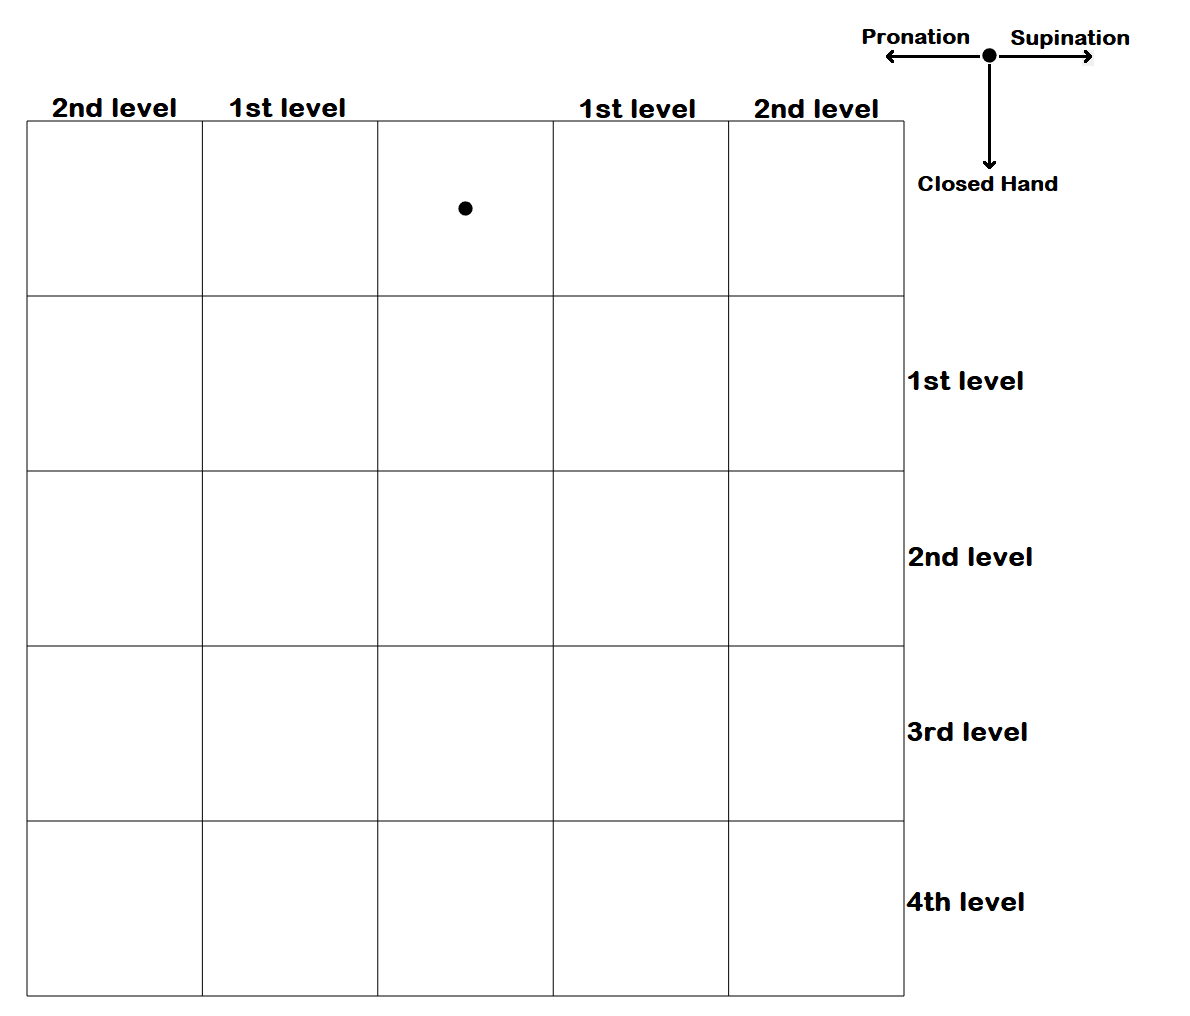
\includegraphics[width=0.45\textwidth]{figures/gridmap2}  
	\caption{Image of the grid map and cursor used in the experiment. Performing supination moved the cursor to the right, pronation moved it to the left and closing the hand moved it downwards. For left handed subjects the rotational movements were reversed. Opening the hand moved the cursor upwards, and was used as a correction movement if needed.}
	\label{fig:meth:gridmap} 
\end{figure}